\section{模块 6 · 追溯修正与最终台账：闸门允许被更强的证据推翻}

模块 5 结束时实例数是 2{,}283，但你在前面已经多次看到最终数字是 \textbf{2{,}267}。
差额来自两批\textbf{追溯修正}（retroactive correction）：
Gate A 判决之后，管线继续往下跑，\textbf{下游步骤算出了 Gate A 当时没有的更强证据}，
据此回头推翻了一批早先的判决。本模块讲这两批修正、一次被否决的``聪明主意''，
以及最后的逐项对账——这部分是汇报里最能体现方法论成熟度的内容。

\subsection{为什么闸门要允许``往回开''}

Gate A 手里只有实例的\textbf{高度}和\textbf{平面形状}。有两类冒牌货靠这两样看不出来：

\begin{itemize}
\item \textbf{茂密的树冠团}：又高（$>$5 米）又紧凑（俯视近圆形），高度、形状都像一栋小楼；
\item \textbf{被树``桥接''的连体楼}：两栋楼中间隔着大树，树冠被错标成建筑点、
      恰好把两栋楼连成一片——看起来就是一栋大楼（步骤 2 的漏网欠分割）。
\end{itemize}

它们的破绽要等\textbf{下游}才显形：第 4 步平面提取会发现树冠``拟合不出像样的平面''；
后续轮廓处理会发现连体楼的屋顶``裂成两大块''。设计选择是：
\textbf{不假装闸门一次判对，而是把下游的新证据回传，逐案重审、修正、记录}
——审计表里这类判决的原因码都带 \texttt{retro}（追溯）字样，全程可查。

\subsection{追溯修正一：22 个树冠假实例}

\textbf{新证据有两条}，都是可计算的分数：
（a）\textbf{植被上下文}：对每个提取出的平面，统计``它所占的 1 米格子（向外扩 1 格）内、
高程落在该平面上下 2 米窗口里的类别 5（植被）点数''与平面自身点数之比。
真屋面身边的植被在窗口之外（比值 $\approx0$）；树冠拟出来的假面则整个泡在同一团
类别 5 点云里（比值远大于 1，记为``植被嫌疑面''）。
（b）\textbf{平面性反馈}：树冠蓬松，点大量归不进任何平面。
把每个实例的``无平面可归的点 $+$ 植被嫌疑面上的点''加起来除以实例总点数，
占比 $\geq 0.90$（几乎整个实例都不像正经屋顶）即成为\textbf{实例级候选}。

按此规则全区捞出 \textbf{24 个候选}，\textbf{逐个人工目验}（俯视图 + 高度剖面）：
\textbf{22 个确认为树冠、整实例剔除}；\textbf{2 个救回}——树下工具棚、单坡车棚这类
真实结构，点稀疏又埋在植被堆里，分数高到 0.94--0.95，目验却一眼可辨是人造物。
连同平面级复核中救下的另 4 个，共 \textbf{6 个实例进入白名单}永久保护。
这 6 个救回案例正说明``规则捞人、人来定罪''不是走过场。
被剔除的 22 个实例照例\textbf{移仓存档}（\texttt{veg\_reclassified.laz}），
原因码 \texttt{reject\_vegetation\_retro} 写回审计表；两项证据分数逐实例/逐面存于
\texttt{instance\_veg.csv} 与 \texttt{plane\_veg.csv}，每个判读都可据表复核。

\subsection{插曲：一个被数据否决的``聪明主意''（负结果）}

处理树冠问题时出现过一个诱人的想法，最终被我们\textbf{用实测数据否决}。
汇报时值得专门讲——它展示``选型靠证据、不靠直觉''。

先补一个知识点：一束激光可以有\textbf{多次回波}（multiple returns）。
激光打到树叶时一部分能量反射（第 1 次回波）、其余能量穿过缝隙继续前进，
可能再打到枝叶（第 2 次）、最后打到地面（最后一次）。所以每个点都带着
``这是第几次回波 / 共几次''的属性。本讲义说的\textbf{中间回波}，操作定义是
``\textbf{回波序号 $<$ 总回波数}''——即多次回波脉冲里\textbf{非最后一次}的回波
（多回波的第 1 次也算在内；不算的只有单次回波与每束脉冲的最后一次）。
树冠的典型特征就是大量中间回波：实测本区\textbf{全部植被（类别 5）点}中
\textbf{94.8\%} 是中间回波，而\textbf{全部被标为建筑（类别 6）的点}中只有
\textbf{10.4\%}——注意这两个比例的分母不同，后面还会用到这一点。

诱人的想法随之而来：\textbf{在单体化之前，把中间回波点统统删掉}，
树冠不就从源头消失了？实测评估给出了两条相反的证据：

\begin{enumerate}
\item \textbf{代价大得离谱}：拿一栋干净的人字顶住宅做案例试验，删中间回波会损失
      该楼 \textbf{9.3\%} 的点（428/4{,}579，图~\ref{fig:echo} 左、中），
      而且\textbf{全部集中在屋檐一圈}——激光束扫到屋檐边缘时会``劈成两半''
      （一半打屋檐、一半继续打到地面），屋檐点因此常是``第 1 次/共 2 次''回波，
      按上面的操作定义正属于中间回波。而屋檐一圈正是建筑\textbf{外轮廓的核心证据}，
      删它等于自毁轮廓。
\item \textbf{收益小得可怜}：对一个真实的树冠污染团（曾被错标成建筑的实例）实测，
      删中间回波只能去掉其中 \textbf{16\%} 的树点（图~\ref{fig:echo} 右）
      ——84\% 的污染原样留下。为什么与 94.8\% 差这么远？这是一次典型的
      \textbf{选择偏差}（selection bias）：我们面对的不是``全体树点''，
      而是\textbf{先被 RandLA-Net 错标成建筑}的那部分树点；模型恰恰倾向把
      ``回波上像表面''的树点——单次或末次回波——错标成建筑，
      于是这个被筛出来的子集\textbf{天然缺乏}中间回波特征。
      94.8\% 描述的是没被错标的大多数，拿它推断被错标的少数，就掉进了坑里。
\end{enumerate}

结论：点级回波预过滤\textbf{否决}——两个案例试验的分母各不相同（一栋楼的全部点 vs
一团污染的树点），不能直接相减比较，但方向一致且都致命：真目标出现集中于屋檐的
\textbf{结构性}损伤，假目标的大头却删不掉。回波属性改记为\textbf{面级}判别的
候选辅助特征（``面级''＝先对一个屋顶平面汇总其内部点的中间回波占比、再整面判断
——目前记录在案、\textbf{尚未进入正式流程}）；树冠假面的正式主兜底是模型装配阶段的
\textbf{拓扑孤立性}：真屋面会通过脊线/落差线与邻面连成拓扑图，树冠假面连不进去。

\begin{figure}[H]
\centering
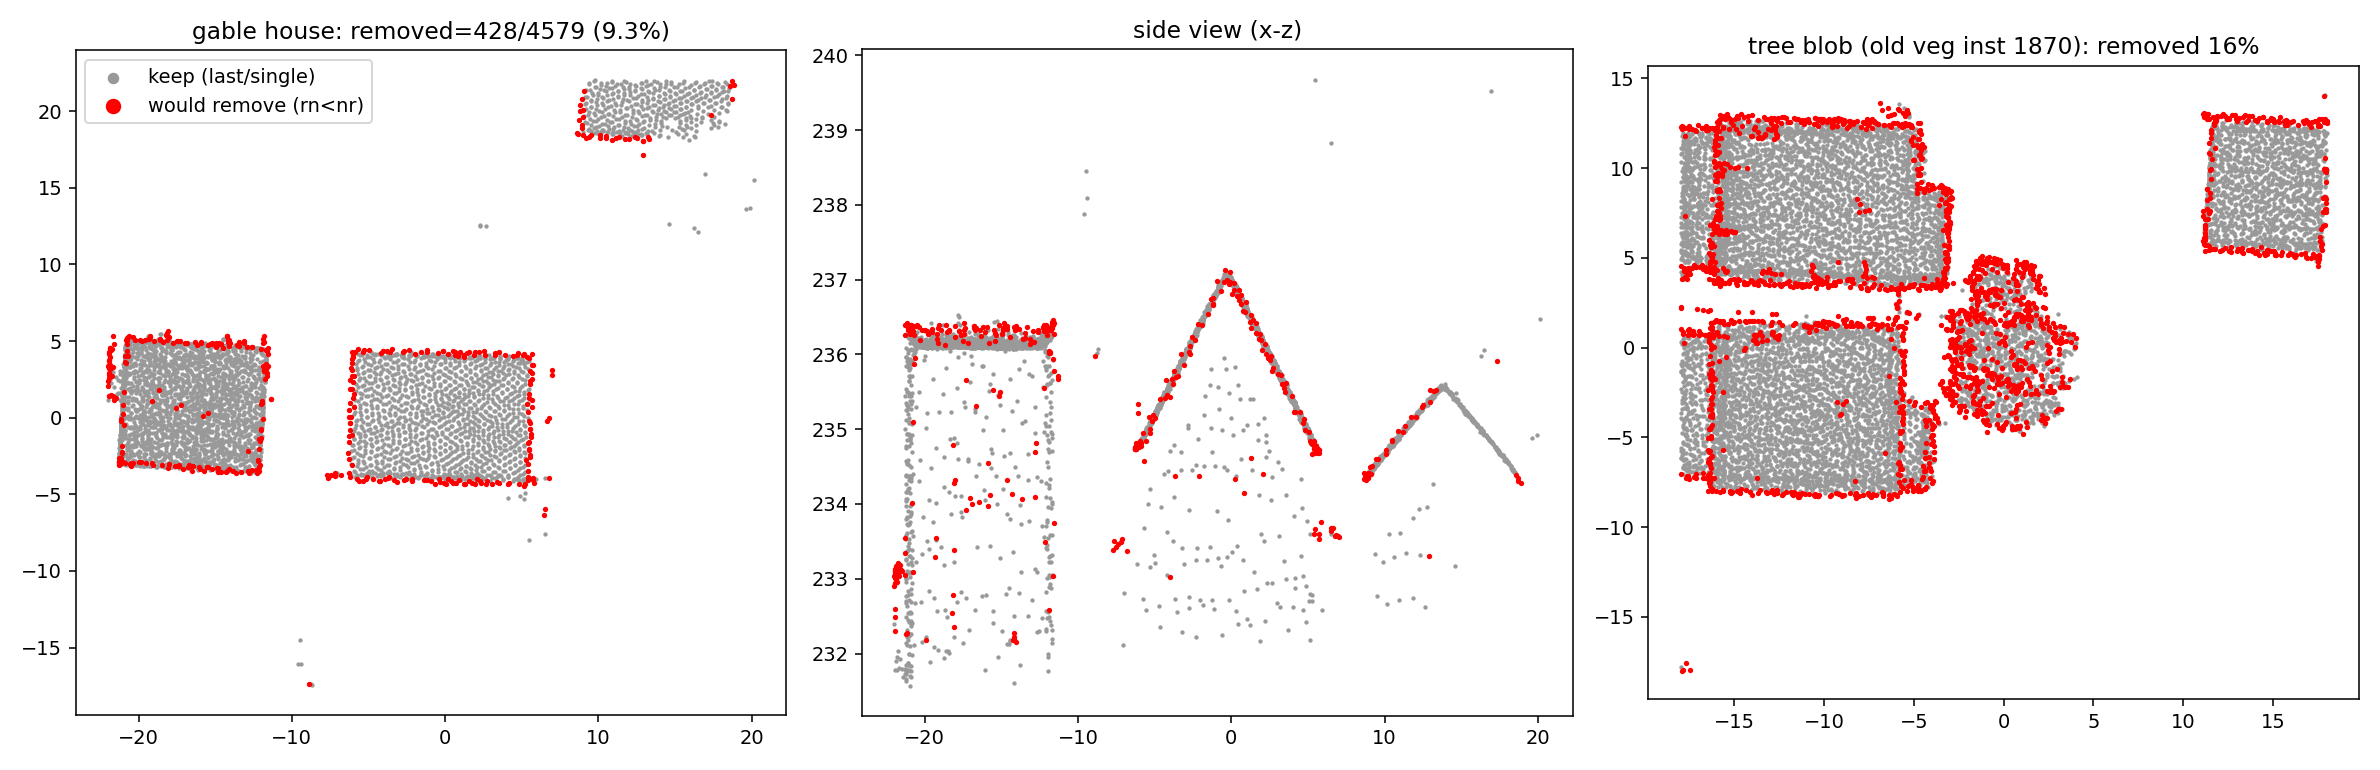
\includegraphics[width=0.98\textwidth]{figs/qa_echo_check.png}
\caption{回波预过滤评估的原始证据（灰 = 保留的单次/末次回波点，红 = 将被删的中间回波点）。
左、中：干净人字顶住宅，428/4{,}579（9.3\%）被删且全部集中在屋檐一圈
（中图侧视可见红点正勾着屋檐边缘）；右：真实树冠污染团，仅 16\% 被删。}
\label{fig:echo}
\end{figure}

\subsection{追溯修正二：6 栋``连体楼''的物理仲裁拆分}

下游轮廓处理阶段发现：少数实例的\textbf{屋顶掩膜}——把该实例的屋顶点投到格子上
得到的黑白图（黑格＝此处有屋顶点）——\textbf{裂成两个互不相连的大块}，
中间隔着被树冠遮挡、没有屋顶点的空白带。
这有两种截然不同的解释，处置完全相反：

\begin{center}
\begin{tabular}{ll}
\toprule
解释 & 正确处置 \\
\midrule
(a) 其实是\textbf{两栋楼}，树把它们桥接了（漏网欠分割） & 拆成两个实例 \\
(b) 是\textbf{一栋大楼}，中段屋顶被树挡住扫不到 & 保持一个实例 \\
\bottomrule
\end{tabular}
\end{center}

肉眼从俯视图上分不出来。我们设计了一个\textbf{物理判据}：

\begin{center}
\fbox{\parbox{0.92\textwidth}{
两栋独立的楼之间是\textbf{露天地面}——激光能从树冠缝隙里穿下去打在地上，
两块之间的``缝走廊''里会出现\textbf{地面（类别 2）点}；而一栋被树遮住中段的大楼，
``缝''的下面是\textbf{实心屋面}，激光穿过树冠碰到的是屋顶，不该出现地面点。
注意证据是\textbf{非对称}的：走廊里\textbf{大量}地面命中是``两栋楼''的强证据；
命中少却不能单独定案（也可能只是树太密、激光下不去）——所以这个判据只用来
\textbf{确认拆分}，不用来单独证明``是一栋''。（还要坦白一点：``类别 2''是第 1 步
模型打的标签，判据的可靠性依赖语义分割对地面的准确率——好在地面是四类里最容易分对的。）
}}
\end{center}

操作：对每个裂成两大块（第二块 $\geq$ 最大块 25\% 面积）的实例，
在两块\textbf{之间}划出走廊——同时距两块都 $\leq3$ 米、又不属于任何一块的格子带
（``同时靠近双方''保证走廊只落在夹缝里）；然后统计：\textbf{分母}＝走廊内全部
1 米格，\textbf{分子}＝其中含类别 2 地面点的格，占比 $\geq 0.35$ 判``两栋楼''。
0.35 是刻意保守的下限——实测中根本没有出现判据附近的灰色案例，分布是干脆的两极：
要么占比极高，要么连两大块都裂不出来。终版审计表（\texttt{split\_verdicts.csv}）里
\textbf{6 个实例命中率 0.96--1.00}（编号 209/217/228/1244/1703/2098，
分别为 1.00/0.96/1.00/1.00/1.00/0.99——几乎每个走廊格都有地面点），
确凿为两栋楼、全部拆分，其中就包括用户在抽查中亲手指认的 228；母实例注销，下游全链重跑。
另有 \textbf{2 个被点名复查的疑似案例}（216/307），检查发现其屋顶掩膜实为一整块
连通区域、根本裂不出两大块（不满足仲裁前提，自然无缝可测），维持单栋判定，证据同样在案。

拆出的 \textbf{12 个新实例编号 2296--2307}。眼尖的读者会发现 2296 与模块 4 的
原编号上限重合：原 2296 号是一个 24.8 m\textsuperscript{2} 的小实例，
已在上一节的树冠追溯中被剔除，编号腾空后被新实例复用——审计表中该编号因此有两行
（旧对象的剔除记录 $+$ 新对象的拆分记录），核对时以判定列区分。

\begin{figure}[H]
\centering
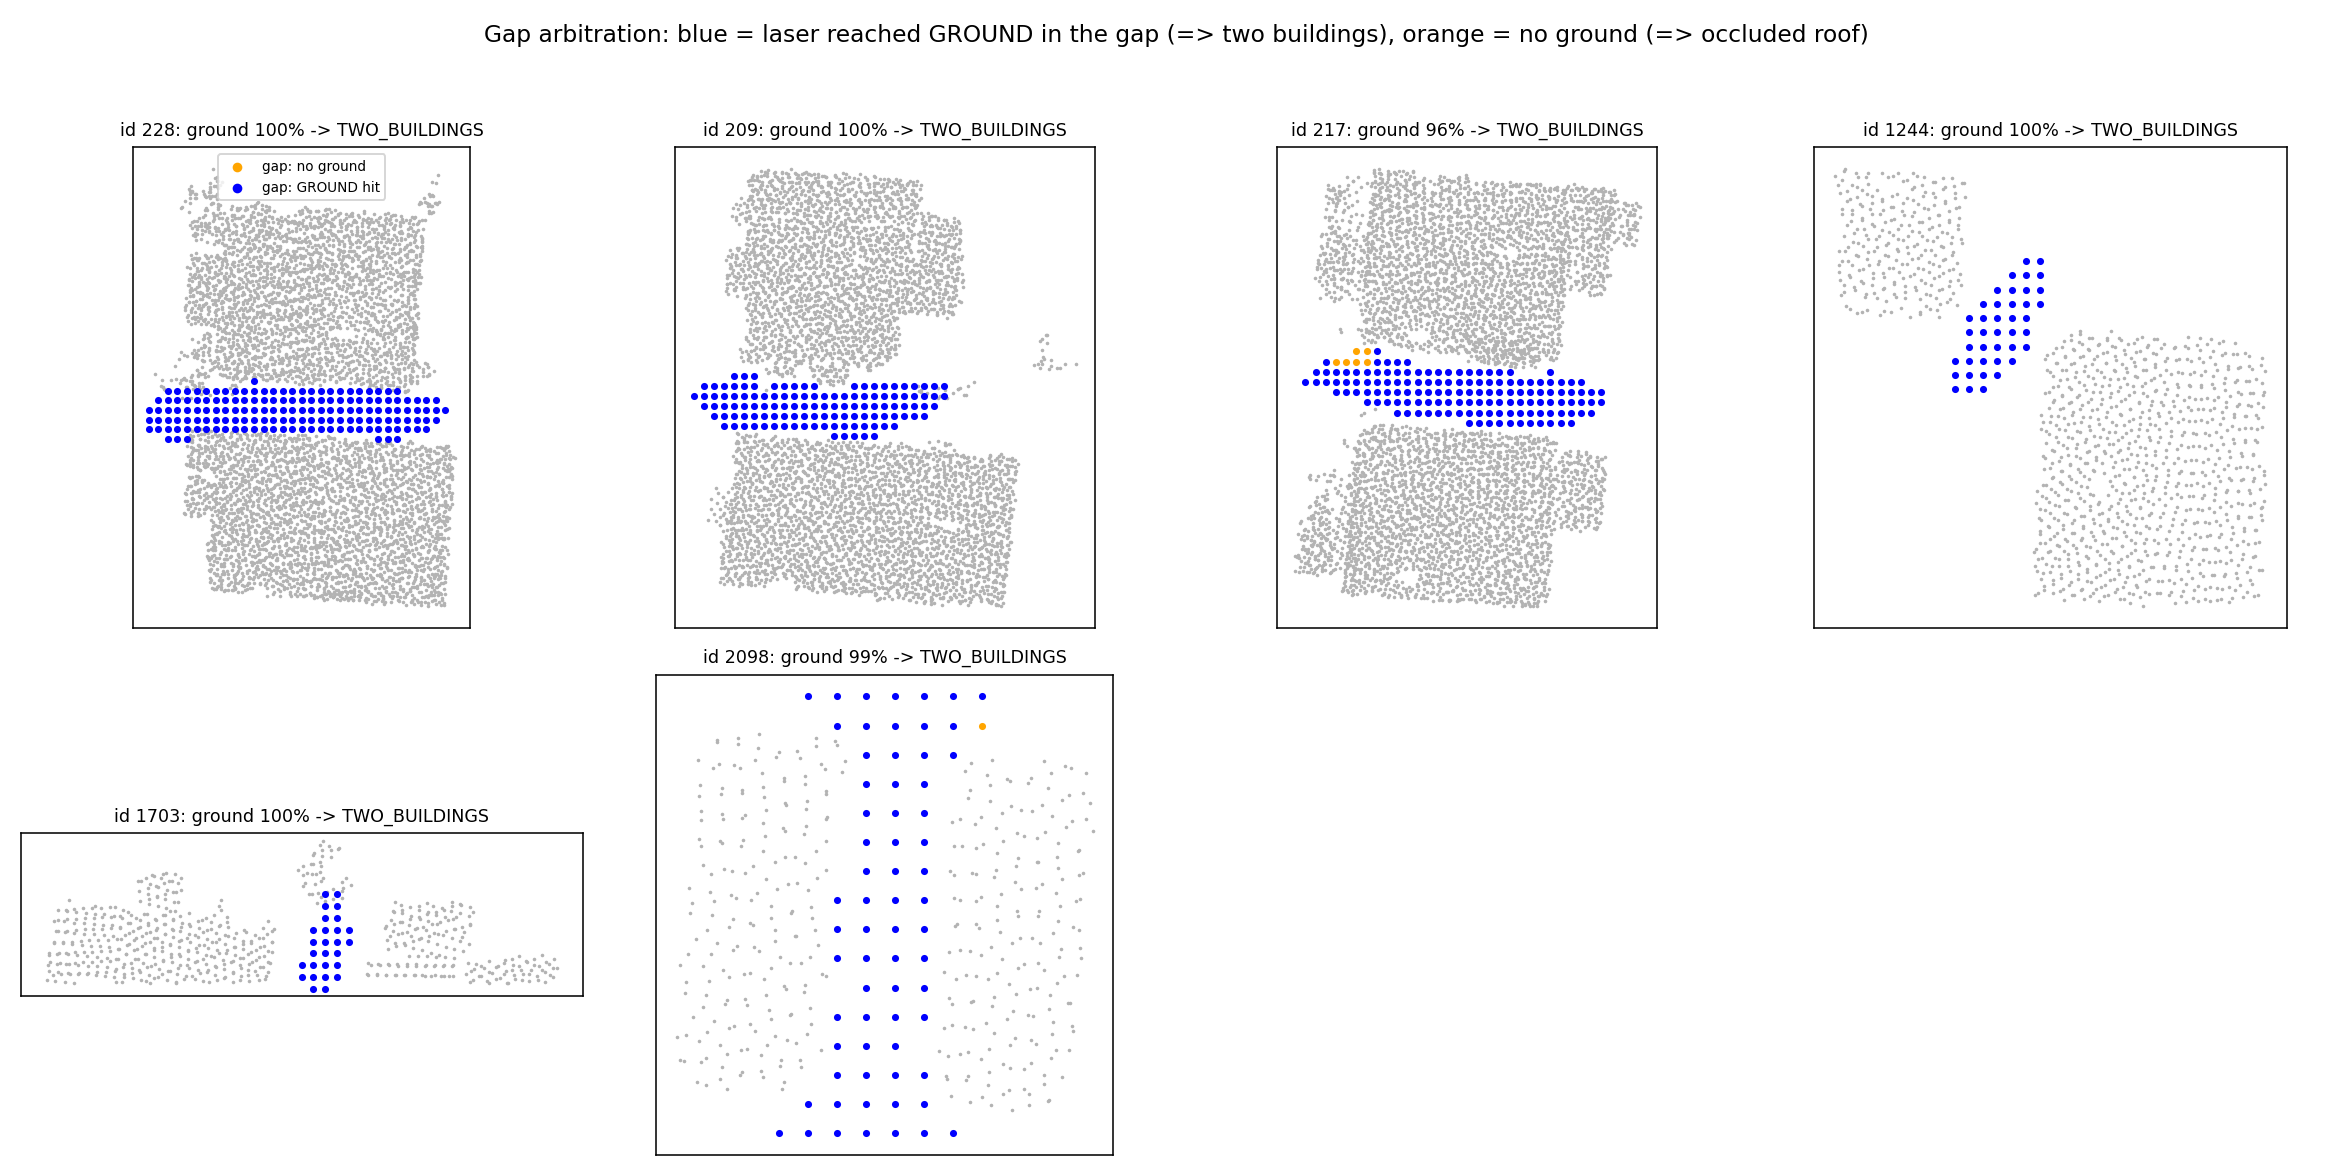
\includegraphics[width=0.95\textwidth]{figs/qa_split_verdicts.png}
\caption{缝内地面命中仲裁：灰 = 屋顶点，蓝 = 走廊内含地面点的格子，橙 = 走廊内无地面点的格子。
六例走廊几乎被蓝点铺满 $\Rightarrow$ 两栋楼（拆分）。两个维持单栋的案例（216/307）
因掩膜连通、无走廊可测，未进入本图。}
\label{fig:split}
\end{figure}

\subsection{最终台账：2{,}296 每一个都有下落}

\begin{numbox}[：逐项对账（数字直接来自审计表 \texttt{instances\_gateA.csv} 的判定列计数）]
\begin{center}
\begin{tabular}{lrl}
\toprule
去向 & 数量 & 说明 \\
\midrule
保留（keep） & 2{,}245 & 判定列为 keep 者——含从未触发规则的多数，也含 A2 复核保留、树冠白名单救回等 \\
细长复核后保留 & 10 & AR$\geq$5 候选中的真实长条建筑（判定列 keep\_reviewed\_ok，模块 5） \\
人工判读剔除 & $-13$ & 桥/匝道/树列/电线，逐个原因码（模块 5） \\
树冠追溯剔除 & $-22$ & 平面性 + 植被上下文 + 目验（本模块） \\
拆分母实例注销 & $-6$ & 缝内地面命中 0.96--1.00（本模块） \\
拆分新生实例 & $+12$ & 编号 2296--2307 \\
\midrule
\textbf{最终干净建筑} & \textbf{2{,}267} & $=2{,}245+10+12$；即 $2{,}296-13-22-6+12$ \\
\bottomrule
\end{tabular}
\end{center}
\end{numbox}

这张表是汇报的``定心丸''：从 2{,}296 到 2{,}267，
每一个消失或新增的编号都有原因码、证据图和存档点云，随时可复查。

\subsection{给 PPT 的建议页序与预答问}

\textbf{建议页序}（每页对应讲义一处，图都是现成的）：
\begin{enumerate}
\item 任务：语义 $\to$ 实例（图~\ref{fig:sem-vs-inst} 重画为 PPT 版）
\item 技术路线一页图：Song \& Jung 骨架 + 分水岭 + 3D BAG 约定（模块 2 总览表）
\item 栅格化与占据规则（图~\ref{fig:raster}）
\item v1 教训：闭运算桥接机理（图~\ref{fig:closing}）+ 检查点复查（图~\ref{fig:checkpoint}）
\item 分水岭拆粘连（图~\ref{fig:erosion-core} + 图~\ref{fig:watershed}；168 拆分战果）
\item Gate A 一页账：HAG（图~\ref{fig:hag}，触发 0 例）；AR 通道 18 候选 $\to$
      8 剔 10 留；A2 通道 25+2 候选 $\to$ 5 剔（图~\ref{fig:solidity}）；合计剔 13
\item 审计总图（图~\ref{fig:gateA}）+ ``规则捞人、人来定罪''原则
\item 追溯修正（上）：树冠 24 候选 $\to$ 22 剔 2 救；回波负结果（图~\ref{fig:echo}）
\item 追溯修正（下）：缝内地面命中仲裁，6 拆、2 不满足前提维持（图~\ref{fig:split}）
\item 台账收官：$2{,}296 \to 2{,}267$ 对账表
\end{enumerate}

\textbf{预答问}（导师高概率提问与推荐答法）：

\begin{itemize}
\item \emph{``为什么不用官方 footprint？''}——研究目标是检验无底图路线的普适性；
      官方 footprint 被有意留作第 9 步的独立评价基准（既当输入又当考卷会让评价失效）。
\item \emph{``为什么不用深度学习做实例分割？''}——无监督路线零训练成本、逐步可审计；
      图聚类新方法（Li 2026）记为候选兜底，本区独栋场景未见必要性。
\item \emph{``0.5 米、$\geq2$ 点这些参数怎么定的？''}——0.5 m 由侧院宽度与点密度共同约束
      （太粗糊缝、太细图斑破碎）；$\geq2$ 点按 30 点/m\textsuperscript{2} 密度下
      0.5 m 格均 7--8 点设定，专杀孤立错点。参数改动都经过检查点复核。
\item \emph{``分水岭会不会把一栋楼错拆成两栋？''}——核有 6 m\textsuperscript{2}
      面积门槛，屋顶毛刺成不了核，从源头压低错拆率；小碎片式的错拆由碎片吸收兜住。
      要诚实承认：``大块对大块''的错拆没有自动纠错（缝内仲裁只负责确认拆分、
      不做反向合并），靠逐楼人工抽查覆盖——本区抽查未发现此类案例。
\item \emph{``删错了怎么办？''}——没有物理删除：全部移仓存档 + 原因码，可整体回滚；
      且删除决定全部经过人工目验，白名单救回 6 例证明流程真实运转。
\item \emph{``树把两栋楼连起来，你怎么发现的？''}——缝内地面命中率：
      激光穿过树冠缝隙会在露天缝里打出地面点，实心屋面下则不会。
      6 例命中 0.96--1.00、无灰色案例，物理判据干脆。
\end{itemize}

\begin{plainbox}[：模块 6 小结（也是全讲义收尾）]
步骤 2--3 的完整故事：863 万建筑点 $\to$ 栅格化 + 连通域（不做闭运算）
$\to$ 分水岭拆 168 处粘连 $\to$ 2{,}296 候选 $\to$ Gate A 规则捞人、人工定罪（$-13$）
$\to$ 下游证据追溯修正（$-22$ 树冠、6 拆 12）$\to$ \textbf{2{,}267 栋干净建筑}，
每一步有论文依据、每一个决定有原因码、每一批数字可对账。
\end{plainbox}
